% IE500 Data Mining - project proposal (max. 4 pages including the title page).
% Based on the LaTeX template of the DWS thesis (dws-templates/thesis.tex).
% Do not change document class, margins, fonts, etc.
\documentclass[a4paper,oneside,bibliography=totoc]{scrbook}

% some useful packages (add more as needed)
\usepackage[utf8]{inputenc}
\usepackage{graphicx}
\usepackage{latexsym}
\usepackage{amsmath}
\usepackage{amssymb}
\usepackage{tabularx}
\usepackage{booktabs}
\usepackage{csquotes}
\usepackage[usenames,dvipsnames]{xcolor}
\usepackage[colorlinks,citecolor=Green]{hyperref} % you may change/remove the colors
\usepackage[bottom]{footmisc} % footnotes below a figure at the bottom of the page
\usepackage{listings} % excerpt of the game file, set as code
\lstset{basicstyle=\ttfamily\footnotesize, columns=fullflexible, keepspaces=true,
  backgroundcolor=\color{black!6}, frame=single, rulecolor=\color{black!30}, framesep=3pt,
  xleftmargin=4pt, xrightmargin=4pt, aboveskip=0pt, belowskip=0pt,
  moredelim={[is][\color{BrickRed}]{@}{@}}} % @...@ marks the blunder

% Team details shown on the first page of the proposal, the final paper and the presentation.
% This is the only place where they have to be edited.
\newcommand{\TeamNumber}{5}
\newcommand{\TeamMembers}{Omar Ahmed Mohamed Taha Radwan, Yeuk Yu Lam,\\ Laith Philipp Sandouk, Arhan Erdogan,\\ Jonas Stammer, Jaden Tan Eden}
\newcommand{\ProjectTitle}{Predicting Blunders in Online Chess}
\newcommand{\ProjectSubtitle}{Can a Blunder in a Lichess Game Be Foreseen Before the Move Is Played?}
\newcommand{\SubmissionDate}{\today}

% Title and date as submitted on 14 October 2026.
\renewcommand{\ProjectTitle}{Predicting Blunders in Online Chess}
\renewcommand{\ProjectSubtitle}{Can a Blunder in a Lichess Game Be Foreseen Before the Move Is Played?}
\renewcommand{\SubmissionDate}{October 14, 2026}

\begin{document}

% Logo: public/logo/lichess.svg of github.com/lichess-org/lila ("only use to refer to lichess.org").
% It is set in a box without height, so that the title block stays where the template puts it.
\frontmatter \titlehead{\centering\raisebox{-\height}[0pt][0pt]{
\includegraphics[height=1.8cm]{lichess_logo}}}
\subject{IE500 Data Mining -- Project Proposal}
\title{\ProjectTitle}
\subtitle{\ProjectSubtitle}
\author{Team \TeamNumber\\[.3em] \TeamMembers}
\date{\SubmissionDate}
\publishers{{\small Submitted to}\\
  Data and Web Science Group\\
  University of Mannheim\\}
\maketitle

\mainmatter

\chapter{Project Proposal}

\section{What is the problem you are solving?}

Chess is more than a game of optimal moves. Human decisions also depend
on time pressure, position complexity, player skill and the demands of
an ongoing game.

A blunder is a serious error that reduces a player's winning chances.
Lichess classifies a move as a blunder when it reduces the
engine-estimated chances by at least 30 percentage
points.\footnote{\href{https://github.com/lichess-org/lila/blob/cf9e10df24b767b3bc5ee3d88c45437ac722025d/modules/analyse/src/main/Advice.scala\#L52}{\texttt{lichess-org/lila}, \texttt{Advice.scala}}}
These chances are derived from Stockfish centipawn evaluations by
a logistic transformation.\footnote{$\text{Win\%} =
50 + 50 \cdot (2 / (1 + \exp(-0.00368208 \cdot
\text{centipawns})) - 1)$;
\url{https://lichess.org/page/accuracy}}
Game files mark blunders with ``??'' (Figure~\ref{fig:blunder}).

% blunder_example.pdf is written by blunder_example.py
\begin{figure}[tb]
  \begin{minipage}[c]{0.255\textwidth}
    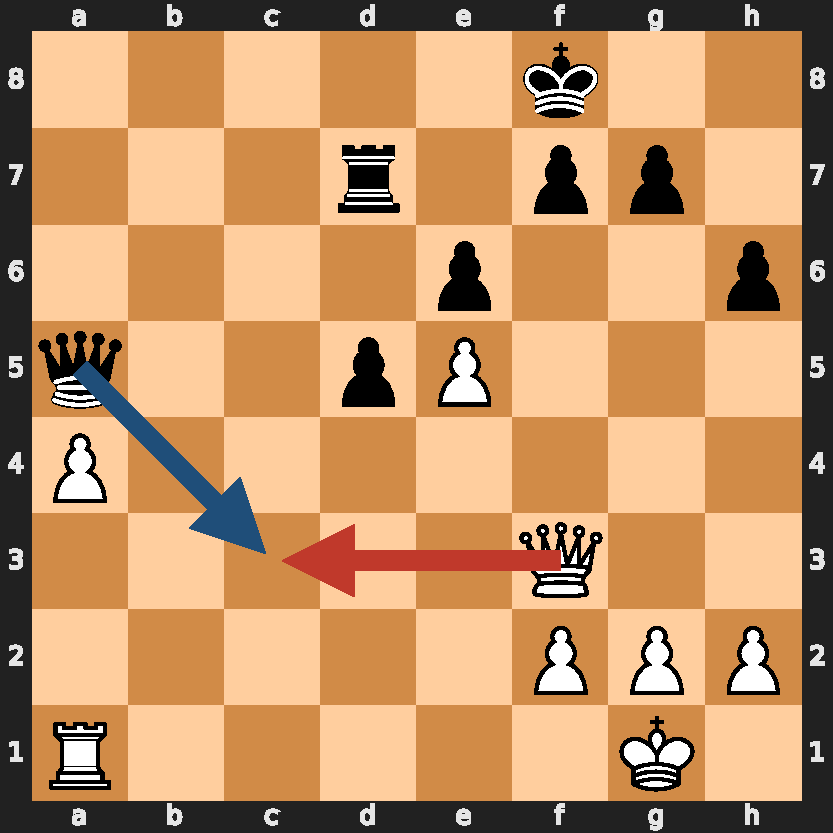
\includegraphics[width=\linewidth]{blunder_example}
  \end{minipage}\hfill
  \begin{minipage}[c]{0.715\textwidth}
\begin{lstlisting}
[WhiteElo "1413"] [BlackElo "1452"] [TimeControl "600+0"]
28. cxd5 { [%eval -0.36] [%clk 0:00:40] }
28... cxd5 { [%eval -0.32] [%clk 0:06:22] }
29. @Qc3??@ { [%eval -9.42] [%clk 0:00:18] }
29... Qxc3 { [%eval -9.41] [%clk 0:06:18] } 0-1
\end{lstlisting}
    \caption{A blunder
      (\href{https://lichess.org/Eh02O2q8}{\texttt{lichess.org/Eh02O2q8}}):
      in a roughly equal position, with 40 seconds left against 6:22,
      White puts the queen on c3 (red), undefended, and Black captures
      it for free (blue).}
    \label{fig:blunder}
  \end{minipage}
\end{figure}

Chess engines such as Stockfish can evaluate any position, but they
assess its strength rather than the likelihood of human error. A
theoretically winning position may still be hard to play under time
pressure. While previous research has examined chess performance and
human mistakes, we investigate whether situational information improves
blunder prediction beyond board evaluations alone. Our research question is:
\emph{Can a machine learning model predict whether a human player
will blunder on their upcoming move, using clock pressure, position
evaluation, player rating and game progression?}

Such predictions could enable personalised warnings and training
diagnostics, give insight into decisions under pressure, and help
spectators assess the risk of blunders.

\section{What data will you use?}
\label{sec:data}

% sloppypar: the two typewriter names cannot be hyphenated and would run into the margin
\begin{sloppypar}
We use the Lichess Open Database
(\href{https://database.lichess.org}{\texttt{database.lichess.org}}),
published under the Creative Commons Zero licence. Our source is
\nolinkurl{lichess_db_standard_rated_2026-09.pgn.zst}, containing
89,616,462 rated standard games from September 2026. As in
Figure~\ref{fig:blunder}, each game has a header with metadata such as
ratings, time control and termination, followed by the moves with remaining
clock times (\texttt{[\%clk ...]}) and, for the approximately 6\% of games
that are analysed, Stockfish evaluations (\texttt{[\%eval ...]}).
\end{sloppypar}

The compressed archive is 29.2~GB, making full local processing
impractical. We will retrieve blocks spread evenly across the month using
HTTP byte-range requests aligned with independently decompressible zstd
frames, and check the edges of each block for split games. We sample whole
games with Stockfish evaluations, with a cap on positions per game so that
very long games do not dominate, up to one million move-level observations.
We then check the rating and time-control mix and stratify if rare groups,
such as classical or very high-rated games, are under-represented.

\section{How will you solve the problem?}
\label{sec:solve}

\textbf{Preprocessing. (1)~Filter (missing values and errors).} We keep only
usable games: bullet to classical, two rated human players, ended normally or
on time, with clock times and Stockfish evaluations. Many games lack
evaluations or clocks, and aborted, bot or truncated games give unreliable
values, so we drop them rather than guess. We also require about 20
half-moves, since very short games are mostly opening noise or early
resignations and do not represent mid-game decision making.

\textbf{(2)~Replay and label.} PGN stores only moves and comments, so we
replay every game with python-chess to rebuild the board before each move.
One example is one position, labelled 1 if the move that follows carries the
``??'' annotation, else 0.

\textbf{(3)~Features (leakage).} The label is defined by the evaluation
change caused by the move, so any feature that sees the move or its aftermath
would reveal the answer. We therefore build about 50 features of the
situation before the move, in six groups: game context (colour, time control,
move number, game phase), ratings of both players, clocks (time left, time
spent on earlier moves, total time used), engine evaluation (win probability,
recent swings), earlier errors of both players, and board complexity
(material, legal moves, possible captures and checks, attacked, undefended
and pinned pieces, king safety). The move itself, the time spent on it, the
result and the termination are never used, and unusually high feature
importance is treated as a leakage alarm. Fatigue cannot be observed
directly, as our blocks do not show a player's full session, so we use
within-game proxies (move number, total time used) and state this as a
limitation.

\textbf{(4)~Cleaning.} Missing values are limited to early-move features that
need history, such as time spent on the previous move; we impute them with
the training median and add an indicator flag. We scale clock times by the
time control, since 30 seconds mean different things in bullet and classical,
and cap evaluations at ten pawns so that mate scores do not distort the
scale. We then standardise and one-hot encode, fitting imputation and scaling
on training data only to avoid leaking test information.

\textbf{(5)~Imbalance.} In a first sample of 88,779 usable games (945,171
positions), 5.5\% of positions are followed by a blunder. We re-measure this
base rate on the final sample, then train on the natural class mix (with and
without class weights) and on a balanced mix (non-blunders undersampled to
50\%); only the training set is resampled. To limit noise from correlated
features, we bin continuous features where useful, drop near-duplicates by a
correlation check, and compare with tree-based feature importance.

\textbf{Algorithms.} Baselines: the blunder rate overall, per speed category
and per rating band, a one-feature rule on the win probability, and a warning
after a substantial opponent error. Symbolic: a CART decision tree.
Non-symbolic: logistic regression, Gaussian naive Bayes, random forest,
gradient-boosted trees (XGBoost) and a small neural network. Hyperparameters
(tree depth, leaf size, number of trees, learning rate, regularisation,
network size) are tuned by stratified 5-fold cross-validation on the training
games. If time allows, we add two extensions: a regression of the centipawn
loss per move, to see how game quality changes throughout a game, and a
k-means clustering of players by error profile, to see whether error
patterns differ with playing style.

\section{How will you measure success?}

\textbf{Split.} We randomly split the games into 80\% training and 20\% test
data, keeping the natural blunder rate. Positions from one game share
ratings, clocks and history, so they stay together to avoid leakage. The
same cross-validation is used to compare models and select prediction
thresholds; the test set is only used for the final evaluation.

\textbf{Measures.} As only 5.5\% of positions are followed by a blunder,
accuracy is misleading: never predicting a blunder already reaches 94.5\%.
Our main metric is Average Precision (AP), which summarises how well a model
finds blunders across all thresholds; a random model, like always predicting
a blunder, achieves about 0.055. We also report precision, recall, F1 and
ROC-AUC, and compare with the baselines of Section~\ref{sec:solve}.

\textbf{Further checks.} Ideally, we would also test whether our models
generalise to later games and unseen players; given our time and computing
resources, we prioritise comparing performance across ratings, time controls
and game phases. We also remove single feature groups, such as clocks or
Stockfish evaluations, to see which contribute most.

\textbf{Success.} The project succeeds if our best model beats the strongest
baseline in AP on the test set and we identify which features are most
useful for predicting blunders.

\section{What do you expect your results to look like?}

We expect the models, boosted trees first, to clearly beat the baselines in
AP, yet most warnings will be false alarms, as a blunder is partly chance;
balanced training should raise recall at the cost of precision. The first
sample already shows patterns. Weaker players blunder more often (7.8\% of
moves below a rating of 1200, 3.9\% from 2000), as do players short of time
(8.2\% with under a twentieth of their time, 4.8\% with over half).
Blunders are rare in the first ten moves (2.2\%) and peak in moves 21 to 30
(7.6\%). The strongest signal is the opponent's last move: if it lost at
least 20 points of win probability, 27.7\% of replies are blunders, against
4.3\% otherwise, because missing the refutation counts as a blunder too. We
therefore expect the evaluation and the earlier errors to matter most when
feature groups are removed, and the decision tree to give readable rules
such as ``the opponent has just erred and the position is sharp: high
risk''.

\end{document}
